\section{Compass\-Search Class Reference}
\label{classCompassSearch}\index{CompassSearch@{CompassSearch}}
{\tt \#include $<$Compass\-Search.h$>$}

Inheritance diagram for Compass\-Search::\begin{figure}[H]
\begin{center}
\leavevmode
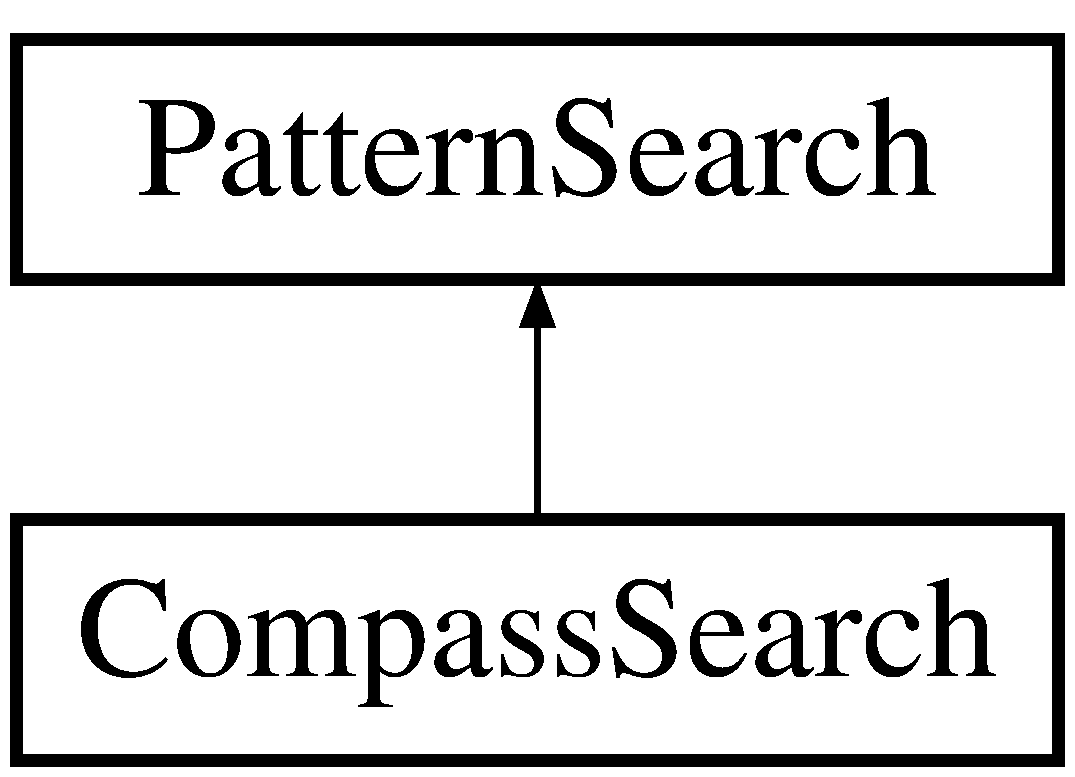
\includegraphics[height=2cm]{classCompassSearch}
\end{center}
\end{figure}
\subsection*{Public Member Functions}
\begin{Indent}{\bf Constructors \& Destructor}\par
\begin{CompactItemize}
\item 
{\bf Compass\-Search} (long number\-Of\-Variables, Vector$<$ double $>$ \&start\-Point)
\item 
{\bf Compass\-Search} (long dim, Vector$<$ double $>$ \&start\-Point, double start\-Step, double stop\-Step, void($\ast$objective)(long vars, Vector$<$ double $>$ \&x, double \&func, bool \&flag, void $\ast$an\_\-obj), void $\ast$input\_\-obj)
\item 
virtual {\bf $\sim$Compass\-Search} ()
\end{CompactItemize}
\end{Indent}
\begin{Indent}{\bf Other public methods}\par
\begin{CompactItemize}
\item 
{\bf Compass\-Search} \& {\bf operator=} (const {\bf Compass\-Search} \&A)
\item 
void {\bf Begin\-Search} ()
\end{CompactItemize}
\end{Indent}
\subsection*{Protected Member Functions}
\begin{CompactItemize}
\item 
void {\bf Exploratory\-Moves} ()
\item 
void {\bf Create\-Pattern} ()
\item 
void {\bf Update\-Pattern} ()
\end{CompactItemize}


\subsection{Detailed Description}
The Compass\-Search class is derived from the {\bf Pattern\-Search}{\rm (p.\,\pageref{classPatternSearch})} class. A compass search checks the positive and negative quardinate vectors for each dimension until improvement in the function values is found. The search then relocates to the improving point and begins again.

\begin{Desc}
\item[Author:]Liz Dolan, The College of William and Mary, 1999, modified by P.L. Shepherd, 7/00 \end{Desc}




\subsection{Constructor \& Destructor Documentation}
\index{CompassSearch@{Compass\-Search}!CompassSearch@{CompassSearch}}
\index{CompassSearch@{CompassSearch}!CompassSearch@{Compass\-Search}}
\subsubsection{\setlength{\rightskip}{0pt plus 5cm}Compass\-Search::Compass\-Search (long {\em number\-Of\-Variables}, Vector$<$ double $>$ \& {\em start\-Point})}\label{classCompassSearch_z3_0}


Constructor. This constructor has two parameters. All it does is call the {\bf Pattern\-Search}{\rm (p.\,\pageref{classPatternSearch})} constructor with the same signature, then change its ID number to 2200.

\begin{Desc}
\item[Parameters:]
\begin{description}
\item[{\em dim}]the dimension of the problem \item[{\em startpoint}]the start point for the search \end{description}
\end{Desc}
\begin{Desc}
\item[See also:]{\bf Pattern\-Search::Pattern\-Search(long dim, Vector$<$double$>$ \&start\-Point)}{\rm (p.\,\pageref{classPatternSearch_z15_0})} \end{Desc}
\index{CompassSearch@{Compass\-Search}!CompassSearch@{CompassSearch}}
\index{CompassSearch@{CompassSearch}!CompassSearch@{Compass\-Search}}
\subsubsection{\setlength{\rightskip}{0pt plus 5cm}Compass\-Search::Compass\-Search (long {\em dim}, Vector$<$ double $>$ \& {\em start\-Point}, double {\em start\-Step}, double {\em stop\-Step}, void($\ast$)(long vars, Vector$<$ double $>$ \&x, double \&func, bool \&flag, void $\ast$an\_\-obj) {\em objective}, void $\ast$ {\em input\_\-obj})}\label{classCompassSearch_z3_1}


Special constructor using void function and object pointers. This constructor merely calls the {\bf Pattern\-Search}{\rm (p.\,\pageref{classPatternSearch})} constructor with the same signature, then change its ID number to 2200.

This constructor takes six input parameters. \begin{Desc}
\item[Parameters:]
\begin{description}
\item[{\em dim}]the dimension of the problem \item[{\em start\-Point}]a Vector of doubles, the starting point for the search \item[{\em start\-Step}]the beginning delta, or lattice step length \item[{\em stop\-Step}]the stopping step length for the search \item[{\em objective}]a pointer to the function to be minimized \item[{\em input\_\-obj}]used to send additional data as needed--will normally be set to NULL. \end{description}
\end{Desc}
\begin{Desc}
\item[See also:]{\bf Pattern\-Search}{\rm (p.\,\pageref{classPatternSearch})}(long dim, Vector$<$double$>$ \&start\-Point, double start\-Step, double stop\-Step, void ($\ast$objective)(long vars, Vector$<$double$>$ \&x, double \& func, bool\& flag, void$\ast$ an\_\-obj), void $\ast$ input\_\-obj) \end{Desc}
\index{CompassSearch@{Compass\-Search}!~CompassSearch@{$\sim$CompassSearch}}
\index{~CompassSearch@{$\sim$CompassSearch}!CompassSearch@{Compass\-Search}}
\subsubsection{\setlength{\rightskip}{0pt plus 5cm}virtual Compass\-Search::$\sim${\bf Compass\-Search} ()\hspace{0.3cm}{\tt  [virtual]}}\label{classCompassSearch_z3_2}


Destructor 

\subsection{Member Function Documentation}
\index{CompassSearch@{Compass\-Search}!BeginSearch@{BeginSearch}}
\index{BeginSearch@{BeginSearch}!CompassSearch@{Compass\-Search}}
\subsubsection{\setlength{\rightskip}{0pt plus 5cm}void Compass\-Search::Begin\-Search ()\hspace{0.3cm}{\tt  [virtual]}}\label{classCompassSearch_z5_1}


{\bf Begin\-Search()}{\rm (p.\,\pageref{classCompassSearch_z5_1})} will call the methods that implement the actual compass search algorithm. \begin{Desc}
\item[Returns:]void \end{Desc}


Implements {\bf Pattern\-Search} {\rm (p.\,\pageref{classPatternSearch_z19_0})}.\index{CompassSearch@{Compass\-Search}!CreatePattern@{CreatePattern}}
\index{CreatePattern@{CreatePattern}!CompassSearch@{Compass\-Search}}
\subsubsection{\setlength{\rightskip}{0pt plus 5cm}void Compass\-Search::Create\-Pattern ()\hspace{0.3cm}{\tt  [protected]}}\label{classCompassSearch_b1}


Initializes the pattern to one that contains one positive and one negative unit vector in each of the compass directions. \begin{Desc}
\item[Returns:]void \end{Desc}
\index{CompassSearch@{Compass\-Search}!ExploratoryMoves@{ExploratoryMoves}}
\index{ExploratoryMoves@{ExploratoryMoves}!CompassSearch@{Compass\-Search}}
\subsubsection{\setlength{\rightskip}{0pt plus 5cm}void Compass\-Search::Exploratory\-Moves ()\hspace{0.3cm}{\tt  [protected, virtual]}}\label{classCompassSearch_b0}


Exploratory Moves does the real work of the compass search. \begin{Desc}
\item[Returns:]void \end{Desc}


Implements {\bf Pattern\-Search} {\rm (p.\,\pageref{classPatternSearch_b1})}.\index{CompassSearch@{Compass\-Search}!operator=@{operator=}}
\index{operator=@{operator=}!CompassSearch@{Compass\-Search}}
\subsubsection{\setlength{\rightskip}{0pt plus 5cm}{\bf Compass\-Search}\& Compass\-Search::operator= (const {\bf Compass\-Search} \& {\em A})}\label{classCompassSearch_z5_0}


Overloaded assignment operator \begin{Desc}
\item[Parameters:]
\begin{description}
\item[{\em A}]the search to be assigned to $\ast$this. \end{description}
\end{Desc}
\begin{Desc}
\item[Returns:]Compass\-Search\& \end{Desc}
\index{CompassSearch@{Compass\-Search}!UpdatePattern@{UpdatePattern}}
\index{UpdatePattern@{UpdatePattern}!CompassSearch@{Compass\-Search}}
\subsubsection{\setlength{\rightskip}{0pt plus 5cm}void Compass\-Search::Update\-Pattern ()\hspace{0.3cm}{\tt  [protected]}}\label{classCompassSearch_b2}


Calls the {\bf Pattern\-Search}{\rm (p.\,\pageref{classPatternSearch})} method \{ {\bf Scale\-Pattern()}{\rm (p.\,\pageref{classPatternSearch_b5})}\} to scale the trial steps by SCALE\_\-FACTOR. SCALE\_\-FACTOR is typically 0.5, so the steplength halves itself. \begin{Desc}
\item[Returns:]void \end{Desc}


The documentation for this class was generated from the following file:\begin{CompactItemize}
\item 
Compass\-Search.h\end{CompactItemize}
